
%% bare_conf.tex
%% V1.4
%% 2012/12/27
%% by Michael Shell
%% See:
%% http://www.michaelshell.org/
%% for current contact information.
%%
%% This is a skeleton file demonstrating the use of IEEEtran.cls
%% (requires IEEEtran.cls version 1.8 or later) with an IEEE conference paper.
%%
%% Support sites:
%% http://www.michaelshell.org/tex/ieeetran/
%% http://www.ctan.org/tex-archive/macros/latex/contrib/IEEEtran/
%% and
%% http://www.ieee.org/

%%*************************************************************************
%% Legal Notice:
%% This code is offered as-is without any warranty either expressed or
%% implied; without even the implied warranty of MERCHANTABILITY or
%% FITNESS FOR A PARTICULAR PURPOSE! 
%% User assumes all risk.
%% In no event shall IEEE or any contributor to this code be liable for
%% any damages or losses, including, but not limited to, incidental,
%% consequential, or any other damages, resulting from the use or misuse
%% of any information contained here.
%%
%% All comments are the opinions of their respective authors and are not
%% necessarily endorsed by the IEEE.
%%
%% This work is distributed under the LaTeX Project Public License (LPPL)
%% ( http://www.latex-project.org/ ) version 1.3, and may be freely used,
%% distributed and modified. A copy of the LPPL, version 1.3, is included
%% in the base LaTeX documentation of all distributions of LaTeX released
%% 2003/12/01 or later.
%% Retain all contribution notices and credits.
%% ** Modified files should be clearly indicated as such, including  **
%% ** renaming them and changing author support contact information. **
%%
%% File list of work: IEEEtran.cls, IEEEtran_HOWTO.pdf, bare_adv.tex,
%%                    bare_conf.tex, bare_jrnl.tex, bare_jrnl_compsoc.tex,
%%                    bare_jrnl_transmag.tex
%%*************************************************************************

% *** Authors should verify (and, if needed, correct) their LaTeX system  ***
% *** with the testflow diagnostic prior to trusting their LaTeX platform ***
% *** with production work. IEEE's font choices can trigger bugs that do  ***
% *** not appear when using other class files.                            ***
% The testflow support page is at:
% http://www.michaelshell.org/tex/testflow/



% Note that the a4paper option is mainly intended so that authors in
% countries using A4 can easily print to A4 and see how their papers will
% look in print - the typesetting of the document will not typically be
% affected with changes in paper size (but the bottom and side margins will).
% Use the testflow package mentioned above to verify correct handling of
% both paper sizes by the user's LaTeX system.
%
% Also note that the "draftcls" or "draftclsnofoot", not "draft", option
% should be used if it is desired that the figures are to be displayed in
% draft mode.
%
\documentclass[conference]{IEEEtran}
% Add the compsoc option for Computer Society conferences.
%
% If IEEEtran.cls has not been installed into the LaTeX system files,
% manually specify the path to it like:
% \documentclass[conference]{../sty/IEEEtran}





% Some very useful LaTeX packages include:
% (uncomment the ones you want to load)


% *** MISC UTILITY PACKAGES ***
%
%\usepackage{ifpdf}
% Heiko Oberdiek's ifpdf.sty is very useful if you need conditional
% compilation based on whether the output is pdf or dvi.
% usage:
% \ifpdf
%   % pdf code
% \else
%   % dvi code
% \fi
% The latest version of ifpdf.sty can be obtained from:
% http://www.ctan.org/tex-archive/macros/latex/contrib/oberdiek/
% Also, note that IEEEtran.cls V1.7 and later provides a builtin
% \ifCLASSINFOpdf conditional that works the same way.
% When switching from latex to pdflatex and vice-versa, the compiler may
% have to be run twice to clear warning/error messages.






% *** CITATION PACKAGES ***
%
%\usepackage{cite}
% cite.sty was written by Donald Arseneau
% V1.6 and later of IEEEtran pre-defines the format of the cite.sty package
% \cite{} output to follow that of IEEE. Loading the cite package will
% result in citation numbers being automatically sorted and properly
% "compressed/ranged". e.g., [1], [9], [2], [7], [5], [6] without using
% cite.sty will become [1], [2], [5]--[7], [9] using cite.sty. cite.sty's
% \cite will automatically add leading space, if needed. Use cite.sty's
% noadjust option (cite.sty V3.8 and later) if you want to turn this off
% such as if a citation ever needs to be enclosed in parenthesis.
% cite.sty is already installed on most LaTeX systems. Be sure and use
% version 4.0 (2003-05-27) and later if using hyperref.sty. cite.sty does
% not currently provide for hyperlinked citations.
% The latest version can be obtained at:
% http://www.ctan.org/tex-archive/macros/latex/contrib/cite/
% The documentation is contained in the cite.sty file itself.






% *** GRAPHICS RELATED PACKAGES ***
%
\ifCLASSINFOpdf
  % \usepackage[pdftex]{graphicx}
  % declare the path(s) where your graphic files are
  % \graphicspath{{../pdf/}{../jpeg/}}
  % and their extensions so you won't have to specify these with
  % every instance of \includegraphics
  % \DeclareGraphicsExtensions{.pdf,.jpeg,.png}
\else
  % or other class option (dvipsone, dvipdf, if not using dvips). graphicx
  % will default to the driver specified in the system graphics.cfg if no
  % driver is specified.
  % \usepackage[dvips]{graphicx}
  % declare the path(s) where your graphic files are
  % \graphicspath{{../eps/}}
  % and their extensions so you won't have to specify these with
  % every instance of \includegraphics
  % \DeclareGraphicsExtensions{.eps}
\fi
% graphicx was written by David Carlisle and Sebastian Rahtz. It is
% required if you want graphics, photos, etc. graphicx.sty is already
% installed on most LaTeX systems. The latest version and documentation
% can be obtained at: 
% http://www.ctan.org/tex-archive/macros/latex/required/graphics/
% Another good source of documentation is "Using Imported Graphics in
% LaTeX2e" by Keith Reckdahl which can be found at:
% http://www.ctan.org/tex-archive/info/epslatex/
%
% latex, and pdflatex in dvi mode, support graphics in encapsulated
% postscript (.eps) format. pdflatex in pdf mode supports graphics
% in .pdf, .jpeg, .png and .mps (metapost) formats. Users should ensure
% that all non-photo figures use a vector format (.eps, .pdf, .mps) and
% not a bitmapped formats (.jpeg, .png). IEEE frowns on bitmapped formats
% which can result in "jaggedy"/blurry rendering of lines and letters as
% well as large increases in file sizes.
%
% You can find documentation about the pdfTeX application at:
% http://www.tug.org/applications/pdftex





% *** MATH PACKAGES ***
%
%\usepackage[cmex10]{amsmath}
% A popular package from the American Mathematical Society that provides
% many useful and powerful commands for dealing with mathematics. If using
% it, be sure to load this package with the cmex10 option to ensure that
% only type 1 fonts will utilized at all point sizes. Without this option,
% it is possible that some math symbols, particularly those within
% footnotes, will be rendered in bitmap form which will result in a
% document that can not be IEEE Xplore compliant!
%
% Also, note that the amsmath package sets \interdisplaylinepenalty to 10000
% thus preventing page breaks from occurring within multiline equations. Use:
%\interdisplaylinepenalty=2500
% after loading amsmath to restore such page breaks as IEEEtran.cls normally
% does. amsmath.sty is already installed on most LaTeX systems. The latest
% version and documentation can be obtained at:
% http://www.ctan.org/tex-archive/macros/latex/required/amslatex/math/





% *** SPECIALIZED LIST PACKAGES ***
%
%\usepackage{algorithmic}
% algorithmic.sty was written by Peter Williams and Rogerio Brito.
% This package provides an algorithmic environment fo describing algorithms.
% You can use the algorithmic environment in-text or within a figure
% environment to provide for a floating algorithm. Do NOT use the algorithm
% floating environment provided by algorithm.sty (by the same authors) or
% algorithm2e.sty (by Christophe Fiorio) as IEEE does not use dedicated
% algorithm float types and packages that provide these will not provide
% correct IEEE style captions. The latest version and documentation of
% algorithmic.sty can be obtained at:
% http://www.ctan.org/tex-archive/macros/latex/contrib/algorithms/
% There is also a support site at:
% http://algorithms.berlios.de/index.html
% Also of interest may be the (relatively newer and more customizable)
% algorithmicx.sty package by Szasz Janos:
% http://www.ctan.org/tex-archive/macros/latex/contrib/algorithmicx/




% *** ALIGNMENT PACKAGES ***
%
%\usepackage{array}
% Frank Mittelbach's and David Carlisle's array.sty patches and improves
% the standard LaTeX2e array and tabular environments to provide better
% appearance and additional user controls. As the default LaTeX2e table
% generation code is lacking to the point of almost being broken with
% respect to the quality of the end results, all users are strongly
% advised to use an enhanced (at the very least that provided by array.sty)
% set of table tools. array.sty is already installed on most systems. The
% latest version and documentation can be obtained at:
% http://www.ctan.org/tex-archive/macros/latex/required/tools/


% IEEEtran contains the IEEEeqnarray family of commands that can be used to
% generate multiline equations as well as matrices, tables, etc., of high
% quality.




% *** SUBFIGURE PACKAGES ***
%\ifCLASSOPTIONcompsoc
%  \usepackage[caption=false,font=normalsize,labelfont=sf,textfont=sf]{subfig}
%\else
%  \usepackage[caption=false,font=footnotesize]{subfig}
%\fi
% subfig.sty, written by Steven Douglas Cochran, is the modern replacement
% for subfigure.sty, the latter of which is no longer maintained and is
% incompatible with some LaTeX packages including fixltx2e. However,
% subfig.sty requires and automatically loads Axel Sommerfeldt's caption.sty
% which will override IEEEtran.cls' handling of captions and this will result
% in non-IEEE style figure/table captions. To prevent this problem, be sure
% and invoke subfig.sty's "caption=false" package option (available since
% subfig.sty version 1.3, 2005/06/28) as this is will preserve IEEEtran.cls
% handling of captions.
% Note that the Computer Society format requires a larger sans serif font
% than the serif footnote size font used in traditional IEEE formatting
% and thus the need to invoke different subfig.sty package options depending
% on whether compsoc mode has been enabled.
%
% The latest version and documentation of subfig.sty can be obtained at:
% http://www.ctan.org/tex-archive/macros/latex/contrib/subfig/




% *** FLOAT PACKAGES ***
%
%\usepackage{fixltx2e}
% fixltx2e, the successor to the earlier fix2col.sty, was written by
% Frank Mittelbach and David Carlisle. This package corrects a few problems
% in the LaTeX2e kernel, the most notable of which is that in current
% LaTeX2e releases, the ordering of single and double column floats is not
% guaranteed to be preserved. Thus, an unpatched LaTeX2e can allow a
% single column figure to be placed prior to an earlier double column
% figure. The latest version and documentation can be found at:
% http://www.ctan.org/tex-archive/macros/latex/base/


%\usepackage{stfloats}
% stfloats.sty was written by Sigitas Tolusis. This package gives LaTeX2e
% the ability to do double column floats at the bottom of the page as well
% as the top. (e.g., "\begin{figure*}[!b]" is not normally possible in
% LaTeX2e). It also provides a command:
%\fnbelowfloat
% to enable the placement of footnotes below bottom floats (the standard
% LaTeX2e kernel puts them above bottom floats). This is an invasive package
% which rewrites many portions of the LaTeX2e float routines. It may not work
% with other packages that modify the LaTeX2e float routines. The latest
% version and documentation can be obtained at:
% http://www.ctan.org/tex-archive/macros/latex/contrib/sttools/
% Do not use the stfloats baselinefloat ability as IEEE does not allow
% \baselineskip to stretch. Authors submitting work to the IEEE should note
% that IEEE rarely uses double column equations and that authors should try
% to avoid such use. Do not be tempted to use the cuted.sty or midfloat.sty
% packages (also by Sigitas Tolusis) as IEEE does not format its papers in
% such ways.
% Do not attempt to use stfloats with fixltx2e as they are incompatible.
% Instead, use Morten Hogholm'a dblfloatfix which combines the features
% of both fixltx2e and stfloats:
%
% \usepackage{dblfloatfix}
% The latest version can be found at:
% http://www.ctan.org/tex-archive/macros/latex/contrib/dblfloatfix/




% *** PDF, URL AND HYPERLINK PACKAGES ***
%
%\usepackage{url}
% url.sty was written by Donald Arseneau. It provides better support for
% handling and breaking URLs. url.sty is already installed on most LaTeX
% systems. The latest version and documentation can be obtained at:
% http://www.ctan.org/tex-archive/macros/latex/contrib/url/
% Basically, \url{my_url_here}.

%*** para suportar acentuação ***
\usepackage[utf8]{inputenc}
%\usepackage[brazil]{babel}
\usepackage[USenglish]{babel}

%*** para suportar tabelas com colunas mergeadas ***
\usepackage{multirow}

%*** Para inclusão de imagens e permitir rotacionar texto ***
\usepackage{graphicx}			% Inclusão de gráficos
\graphicspath{ {./} }			% localizando as imagens
\usepackage{multicol}

\usepackage{url}
\usepackage{enumitem}
\usepackage{comment}

%*** Para ajustar a largura das colunas e para multilinhas nas células ***
\usepackage{array}
\newcolumntype{L}{>{\centering\arraybackslash}m{0,75cm}}
\newcolumntype{M}{>{\RaggedLeft\arraybackslash}m{3cm}}

% *** Do not adjust lengths that control margins, column widths, etc. ***
% *** Do not use packages that alter fonts (such as pslatex).         ***
% There should be no need to do such things with IEEEtran.cls V1.6 and later.
% (Unless specifically asked to do so by the journal or conference you plan
% to submit to, of course. )

\usepackage{float}

\usepackage{xcolor}
\newcommand{\marcos}[1]{{\color{blue}{MARCOS: #1}}}
\newcommand{\marcosT}[1]{{\color{red}{TODO: #1}}}
\newcommand{\marcosR}[1]{{\color{brown}{COMMENT: #1}}}
\newcommand{\fancyname}{Dizang }
\newcommand{\fancynameX}{\fancyname}

%shortcuts
\newcommand{\xfig}{
\includegraphics[scale=0.007]{x.png}}
\newcommand{\cfig}{
\includegraphics[scale=0.015]{check.png}}
\newcommand{\rot}[1]{\rotatebox{90}{#1}}
\newcommand{\urls}[1]{{\footnotesize{\url{#1}}}}

% correct bad hyphenation here
\hyphenation{op-tical net-works semi-conduc-tor}


\begin{document}
%
% paper title
% can use linebreaks \\ within to get better formatting as desired
% Do not put math or special symbols in the title.
%\title{Coletando dados de memória de máquina em nuvem para análise forense de ataques de injeção de código}
\title{\fancynameX: A solution for collecting forensic evidences of cloud malware injection attack}


% author names and affiliations
% use a multiple column layout for up to three different
% affiliations
\author{\IEEEauthorblockN{Hamilton J. S. Fonte II, Marcos A. Simplicio Jr., Edson S. Gomi}
\IEEEauthorblockA{
Escola Politécnica, Universidade de São Paulo (USP)
São Paulo, SP, Brasil\\
Email: hamiltonii@gmail.com, mjunior@larc.usp.br, gomi@usp.br}
%\and
%\IEEEauthorblockN{Marcos A. Simplicio Jr.}
%\IEEEauthorblockA{
%Escola Politécnica -- Universidade de São Paulo (USP)
%São Paulo, SP, Brasil\\
%Email: mjunior@larc.usp.br}
}

% conference papers do not typically use \thanks and this command
% is locked out in conference mode. If really needed, such as for
% the acknowledgment of grants, issue a \IEEEoverridecommandlockouts
% after \documentclass

% for over three affiliations, or if they all won't fit within the width
% of the page, use this alternative format:
% 
%\author{\IEEEauthorblockN{Michael Shell\IEEEauthorrefmark{1},
%Homer Simpson\IEEEauthorrefmark{2},
%James Kirk\IEEEauthorrefmark{3}, 
%Montgomery Scott\IEEEauthorrefmark{3} and
%Eldon Tyrell\IEEEauthorrefmark{4}}
%\IEEEauthorblockA{\IEEEauthorrefmark{1}School of Electrical and Computer Engineering\\
%Georgia Institute of Technology,
%Atlanta, Georgia 30332--0250\\ Email: see http://www.michaelshell.org/contact.html}
%\IEEEauthorblockA{\IEEEauthorrefmark{2}Twentieth Century Fox, Springfield, USA\\
%Email: homer@thesimpsons.com}
%\IEEEauthorblockA{\IEEEauthorrefmark{3}Starfleet Academy, San Francisco, California 96678-2391\\
%Telephone: (800) 555--1212, Fax: (888) 555--1212}
%\IEEEauthorblockA{\IEEEauthorrefmark{4}Tyrell Inc., 123 Replicant Street, Los Angeles, California 90210--4321}}




% use for special paper notices
%\IEEEspecialpapernotice{(Invited Paper)}




% make the title area
\maketitle

% As a general rule, do not put math, special symbols or citations
% in the abstract
\begin{abstract}
Cloud architectures are increasingly more common, as is the number of security problems involving this technology. 
%
Unfortunately, due to the volatile nature of resources in the cloud, the collection of evidences for forensic analysis has faced practical and legal challenges.
%
With a technical focus, this work analyzes proposals aimed at meeting the challenges posed by the collection of evidences in the cloud, discusses their limitations and presents a solution to overcome them.
%
The proposal specifically focuses on the reproducibility of the collection process, without violating jurisdictions or the privacy of those not involved in the investigation.

\end{abstract}

% no keywords




% For peer review papers, you can put extra information on the cover
% page as needed:
% \ifCLASSOPTIONpeerreview
% \begin{center} \bfseries EDICS Category: 3-BBND \end{center}
% \fi
%
% For peerreview papers, this IEEEtran command inserts a page break and
% creates the second title. It will be ignored for other modes.
\IEEEpeerreviewmaketitle

\section{Introduction}

%==== CONTEXTO GERAL: Nuvem e volatilidade de VMs ====
%
Visualization techniques, replication of services and resource sharing among multiple users (multitenancy) provide the computational clouds with high scalability \cite{Morsy_Cloud_Security:2010}.
%
Yet these mechanisms also lead to the volatility of the virtual resources that execute the applications.
%
After all, when submitted to a high load, an application hosted in the cloud may create clones of the virtual machines (VMs) hosting it and balance the load between them, seeking to meet the demand without harming the quality of the service offered. 
%
After this peak, the cloned VMs are usually deactivated, their resources are released and the system returns to the previous capacity, preventing unnecessary costs.


%==== CONTEXTO ESPECÍFICO + PROBLEMA GERAL: Forense na nuvem vs. volatilidade + multitenancy + multidomains ====
%
Despite interesting from the efficiency and cost viewpoints, from the forensic point of view, the volatility of the cloud causes problems in case of attacks.
%
For example, in case one of the virtual processing instances temporarily created undergoes threats that act directly on its memory, without leaving traces in disks (e.g. log files), the evidences of this event may be completely lost after they are deactivated and their resources are released.
%
This difficulty is further aggravated by aspects such as multitenancy and multi-jurisdiction, typical of cloud solutions \cite{Bash_Adv_in_Forensics:2015}.
%
Particularly, the multitenancy aspect hinders identifying the hardware executing the applications of interest; since it is shared by a number of users, removing them for analysis could lead to a violation of privacy of the users not related to the investigation. 
%
Moreover, the distributed nature of the cloud may lead to allocating information relevant to the investigation in different countries, thus hindering obtaining this information, especially when there are no cooperation agreements among the entities involved \cite{Dykstra_Acquiring_for_IAAS:2012}.
%
Combined, these characteristics hinder collection of evidences with the necessary credibility so that they can be accepted in legal processes, which require respect to privacy, to the jurisdiction and to the chain of custody, as well as to the reproducibility of the collection process \cite{Rahman_Live_Forensics_Techniques:2015}.


%==== O QUE EXISTE E PORQUE NÃO É SUFICIENTE: ??? ====
%
Although the literature presents solutions aimed at collecting information in the cloud for forensic analysis, most of them approach collection, transport and storage in an isolated manner.
%
Works such as \cite{Dykstra_FROST:2013} and \cite{Reichert_Auto_acquisition:2015} deal with factors such as multitenancy and multi-jurisdiction, discussing forms of collecting and preserving evidence outside the cloud.
%
Works such as \cite{George_DF2CE:2012} concentrate on forensic analysis to collect evidence from VMs while they are being executed, whereas works such as \cite{Sang_Log_approach:2013} deal with guaranteeing the chain of custody for transporting the evidence.
%
However, none of the proposals identified (1) describe how data are collected and stored observing the chain of custody, and (2) allow the conditions for reproducing the evidence collection process even if a virtualized resource is removed.



%==== O QUE FAZEMOS: Ataques de injeção ====
%
This work aims to overcome these limitations, presenting a proposal focusing on: (1) the reproducibility of the collection process, (2) establishing a link between the evidence collected and its origin, (3) preserving the jurisdiction and the privacy of those not involved in the investigation.
%
In sum, the solution described provides a way of correlating evidences and their virtual origin so as to preserve their credibility and thus contribute to their acceptability in a legal process.
%
Lastly, \textit{Incident Management}, which increasingly shares processes and tools with \textit{Digital Forensics}, may benefit from a ready-to-use solution for collecting and preserving evidences at the \textit{preparation for the incident} stage. It should also be able to preserve evidences for the \textit{post-incident} stage, thus making it unnecessary to be concerned with their partial or total loss at the \textit{detection and analysis stages}.
%
For this, the system is supposed to be monitored and executed within a cloud resource univocally identifiable.
%
The solution specifically targets code injection attacks \cite{Case_Memory_Forensics:2014}, seeing that, when these are used against the cloud architecture, they leave no traces when virtual processing resources are deactivated and their memory is released \cite{Vomel_Memory_Acquisition:2013}, \cite{Case_Memory_Forensics:2014}.
%


This paper is organized as follows.
%
Section \ref{sec:cloud} briefly discusses cloud solutions and their characteristics.
%
Section \ref{sec:related} analyzes the works related to the forensic memory area.
%
Section \ref{sec:proposal} details the solution proposed and assesses how it deals with the target challenges of this work. 
%
Section \ref{sec:conclusion} presents the conclusions.



\section{Adoption of Cloud Architecture and Containers}
\label{sec:cloud}


A computational cloud is an infrastructure model in which resources shared at a configurable number, accessible via net, are allocated and removed by a service provider with minimum management effort \cite{NIST2011}.
%
There are three main models for trading use in the cloud \cite{NIST2011}: software as a service (SaaS), in which the software to be used by the client is provided; platform as a service (PaaS), in which an environment is provided for clients to develop, test and execute their software; and the most pertinent type for this work, infrastructure as a service (IaaS), in which basic computational resources are provided, such as processing and memory, generally in a virtualized way.


The virtualization of resources in the cloud, despite traditionally conducted by means of VMs, has also increasingly been peformed in the form of containers.
%
According to a study conducted in 2016 with 235 companies having software development as their end activity or as a support to the end activity \cite{container-survey:2016}, 76\% of the respondents use containers to improve the efficiency of the development process and in their architecture of cloud micro-services.
%
Differently from VMs, which involve creating a virtual hardware and also a O.S. on top of the native system, the virtualization with containers is conducted at the level of the native O.S., which has a simpler implementation, thus eliminating layers between the application executed and the physical hardware.
%
A technology widely used for this purpose is the Linux Containers (LXC), which takes advantage of functionalities such as \textit{cgroups} and \textit{namespacing} of the Linux kernel to help managing and isolating virtual resources.



\section{Related works}
\label{sec:related}

There are a number of aspects related to forensic analysis in the cloud, going from information collection to guaranteeing the evidence chain of custody.
%
For a better structured discussion of the works available in the literature, summarized in Table \ref{tab:related-work}, they are presented as follows, based on the different aspects they approach.

\begin{table}[htb!]
\centering
\caption{Comparison of solutions for collecting memory information from cloud machines for forensic analysis}
\label{tab:related-work}
\renewcommand{\arraystretch}{2}
\begin{tabular}{p{3.0cm}|L|L|L|L}
\cline{2-5}
\textbf{}															& \rotatebox{90}{\textbf{Is the collection continous?}}      & \rotatebox{90}{\textbf{Can it reproduce the process without the VM?}} & \rotatebox{90}{\textbf{Does it guarantee the chain of custody?}}     		& \rotatebox{90}{\textbf{Does it preserve jurisdiction and privacy?}}          \\ \hline
\fancyname (this proposal)						& \cfig	  & \cfig               & \cfig                  & \cfig                             \\ \hline
\cite{George_DF2CE:2012}							& \xfig		  	& \xfig                   & \xfig                      & \cfig                             \\ \hline
\cite{Poisel_VMI:2013}								& \xfig       & \xfig                   & \xfig                      & \cfig                             \\ \hline
\cite{Dykstra_FROST:2013}							& \xfig       & \xfig                   & \xfig                      & \cfig                             \\ \hline
\cite{Do_Desafio:2014}								& \xfig		    & \xfig                   & \xfig                      & \cfig                             \\ \hline
\cite{Reichert_Auto_acquisition:2015}	& \xfig  	    & \xfig                   & \cfig                  & \cfig                             \\ \hline
\cite{Sang_Log_approach:2013}					& \cfig   & \xfig	             			& \cfig                  & \cfig                             \\ \hline
\cite{Dolan-Gavitt_Semantic_Gap:2011}	& \xfig       & \xfig                   & \xfig                      & \cfig                             \\ \hline
\cite{Aljaedi_Comparative:2011}				& \xfig       & \xfig                   & \xfig                      & \cfig                             \\ \hline
\cite{Dezfouli_Backup_approach:2012}	& \cfig   & \xfig                   & \xfig                      & \cfig                             \\ \hline
\cite{VanBaar_FAAS:2014}							& \cfig   & \xfig                   & \cfig                  & \cfig                             \\
\end{tabular}
\end{table}



\subsection{Accessing and collecting information about memory in the cloud}

Different works on forensic analysis in the cloud concentrate on collecting data “after the fact”, i.e., after the intrusion has been detected \cite{Reichert_Auto_acquisition:2015,Poisel_VMI:2013,Dykstra_FROST:2013,George_DF2CE:2012,Sang_Log_approach:2013}. 
%
The collection processes described in those works can be started manually or automatically, by integrating them with an intrusion detection mechanism. 
%
In the specific case of volatile memory, that form of collection cannot describe what the memory was like before the intrusion, since the process is only activated after the attack has been detected. 
%
This limitation can be harmful to the investigation, given that some analyses depend exactly on their ability to compare two moments of the memory \cite{Case_Memory_Forensics:2014}. 
%
Among the works studied, the only proposal found that considers this need is \cite{Dezfouli_Backup_approach:2012}, which proposes that the data are stored in the very equipment under analysis.
%
Unfortunately, however, the application of this approach to the cloud scenario is not very viable, since it can lead to losing important information in case the VM or the container comes to be deactivated and has its resources released.
%

There are also works aimed at collecting information during the system execution, in which data are constantly collected with no distinction between what happened before or after the event of interest.
%
This is the case of works such as \cite{Poisel_VMI:2013,Dykstra_FROST:2013,Sang_Log_approach:2013}, which adopt the strategy of isolating and halting the VM for then conducting the collection process. 
%
Albeit interesting, the approaches described in these works may lead to a massive volume of data collected, besides not treating the scenario from which evidence has to be collected when the virtual resources containing the information are released.


\subsection{Ability to reproduce the process and to obtain the same results}

If, during a forensic analysis, different analysts obtain distinct results when executing the same collection procedure, the evidence generated has no credibility and may come not to be accepted in a legal process. 
%
For this reason, the reproducibility of the collection process is an important part in evidence generation for forensic analysis.
%
None of the proposals currently found in the literature allows this reproducibility in cloud scenarios in which VMs or containers are deactivated and their physical resources are released; they all depend on the existence of the virtual resource for repeating the collection process.


\subsection{Not violating the privacy or jurisdiction of the parts not involved in the investigation}

In a public cloud environment, removing the hardware for later analysis may lead to violating the privacy of users, once this scenario multitenancy makes the same physical machine store information about different clients, some of which may not be involved in the investigation in course.
%
Different works in the literature adequately deal with this issue using two major strategies: the first, adopted by \cite{Reichert_Auto_acquisition:2015,George_DF2CE:2012,Poisel_VMI:2013,Dykstra_FROST:2013}, consists in collecting data pertinent to the investigation and in storing them outside the cloud.; the second, employed in \cite{Sang_Log_approach:2013}, which consists of a specific case of \cite{George_DF2CE:2012}, depends on the cooperation of the cloud service provider for obtaining  the information necessary to the investigation. 
%
Yet depending on the cloud service provider is not a recommended strategy because (1) the volume of user's data may force the providers to limit the size of the logs stored, and (2) in case unavailability caused by an attack occurs, the goal of the provider will be that of restoring the service, rather than preserving evidences \cite{Clarke_Review_of_Challenges:2015}. 



\section{Solution proposed: \fancyname}
\label{sec:proposal}

This proposal aims mainly at collecting memory from virtual computational resources so as to succeed in: 
(1) identifying the evidence source, even if the virtual resource no longer exists; 
(2) describing the system before and after the incident;
(3) transporting and storing the memory collected so as to guarantee its integrity and confidentiality; and
(4) not violating the jurisdiction and privacy of other users that might have resources allocated in the same physical server.
%
The solution here presented, called Dizang, is described in detail as follows.


\subsection{Description}
\label{sec:proposal-desc}

In computational systems executed on a physical infrastructure (i.e., non-virtualized), a direct association can be made between any resource, such as memory information, disk image or packets travelling in the network, and their corresponding origin.
%
In systems built in a virtual infrastructure, especially when it is self-scalable, the computational resources are highly volatile and can thus be removed at any time.
%
To succeed in correlating a piece of evidence to its volatile origin, this implementation uses Linux containers (LXC) to persist in the source-evidence relationship.
%
Although a container is a type of software, and is thus also volatile, each image compiled and its execution in the form of a container are normally linked to a hash that univocally identifies this relationship.
%
The container also allows more precisely identifying the source of a piece of evidence, once it is possible to divide the parts of a system into containers; for example, one container for the engine of dynamic web pages (e.g. \textit{Apache}), another with business logics (e.g. \textit{Golang}) and a third one for a database (e.g. \textit{Cassandra}).


Memory copy is not an atomic activity, since it is executed jointly with other processes.
%
Hence, in case one of these processes is a malicious code erasing traces of its existence from the container memory, possibly important information may eventually be lost. 
%
Aiming to make the memory copy process more atomic, \fancyname temporarily interrupts the execution of the container, makes a copy of its memory and then resumes its execution. 
%
This technique, similar to that adopted by \cite{Rafique_Static_Live_Digital_Forensics:2013} for VMs, produces a photograph of the container volatile memory; this allows its analysis at a repose state, that is, without the need of having the container at work.
%
When conducting the data collection at adequate time intervals, it is possible to build the history of the memory state during its execution in the container.
%

Most of the forensic techniques currently most widely employed are directed to obtaining information in its totality, be it via bit by bit copy, be it by obtaining the physical hardware \cite{Simou_Cloud_Chlng:2014} \cite{Bem_Past_Present_Future:2008}. 
%
Even though these techniques may sound interesting at first, many times they are eventually responsible for a problem: the growing volume of information investigators have to analyze \cite{Quick_Increase_Volume_Impact:2014}.
%
To mitigate this difficulty, \fancyname adopts two strategies. The first is defining a volume of data that may be considered enough for conducting an investigation; the second is defining a maximum age for the evidence while the system works under normal conditions, i.e., when it is not under attack.
%
To detect and to analyze intrusions in the processes memory, it is necessary to have a copy of the memory before and after the intrusion \cite{Case_Memory_Forensics:2014}. 
%
The solution proposed thus implements a window of memory photographs covering a pre-defined time interval, as illustrated in Fig. \ref{fig:janela}. 
%
In normal operation conditions, the pieces of evidence are collected with a certain periodicity and collections reaching a given age are discarded.
%
In contrast, after an attack event is detected, (e.g. by an intrusion detection system), \fancyname stops discarding the oldest collections from the monitoring log, enabling to know the system before and after the attack and hence assess its evolution.
%

\begin{figure}[htb!]
\footnotesize
\caption{Sliding window of evidence collection}
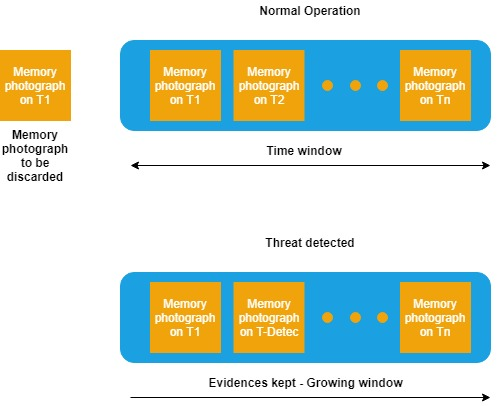
\includegraphics[scale=0.45]{janela_ieee-eng.jpg}
\centering
\label{fig:janela}
\end{figure}

To persist in the evidence-origin relationship and to guarantee its integrity, this proposal calculates the pair hash [evidence, container image identifier] and stores the triple [hash, container image identifier, evidence].
%
To prevent possible problems with the storage of these data in countries with different jurisdictions from those in which they must be applied in the investigation in question, the evidence collected is stored in a physical place outside the cloud, after being transported by a safe channel (e.g. via \textit{Transport Layer Security} – TLS \cite{DierksT2008}).
%

\subsection{Implementation}
\label{sec:proposal-impl}

\begin{figure}[htb!]
\footnotesize
\caption{General architecture of the \fancyname solution}
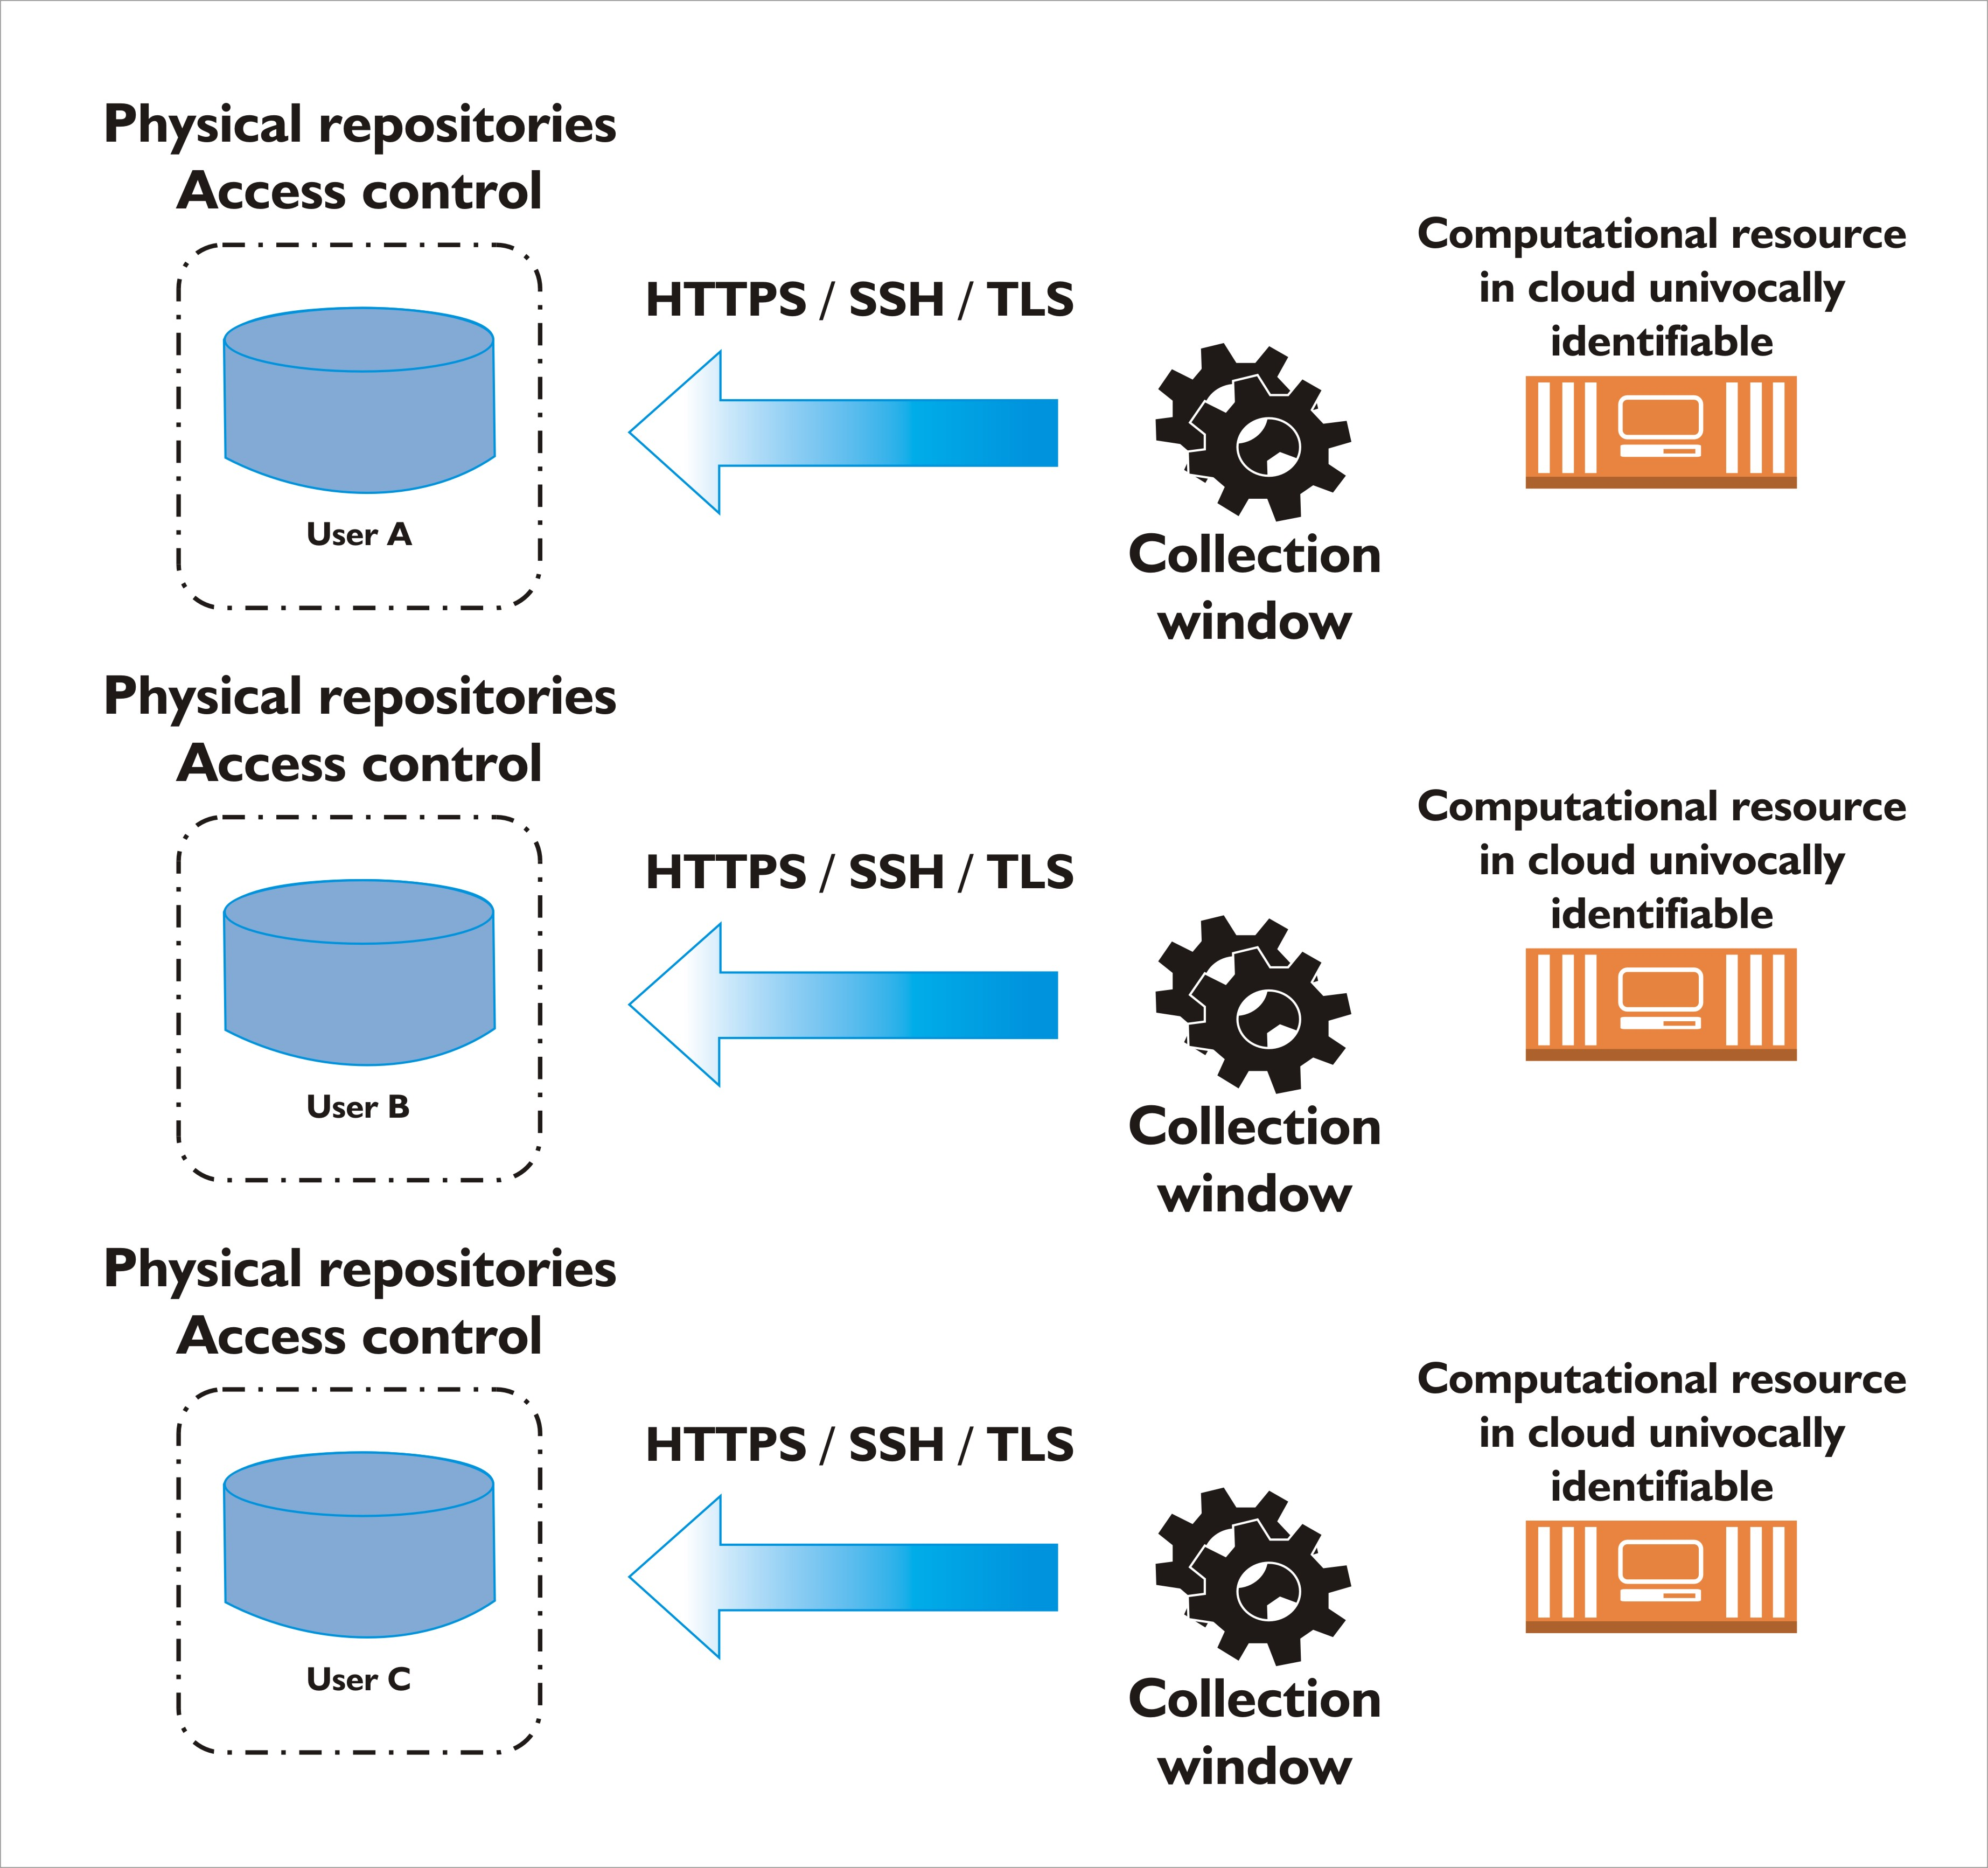
\includegraphics[scale=0.31]{solucao-eng.jpg}
\centering
\label{fig:Solucao}
\end{figure}


The methods proposed were implemented in a test platform aiming to assess the \fancyname efficacy in collecting the memory information from the containers in a reproducible way, without violating jurisdictions or users’ privacy.
%
The solution, illustrated in Fig. \ref{fig:Solucao}, consisted in creating a t2.micro instance in the Ohio zone of the AWS with 3.3 Mhz, 1Gb RAM and 64-bit operational system. 
%
At this AWS instance, Docker Engine 1.10 and API Docker 1.21 were installed, from which 3 containers were created, executing nginx 1.0 at different ports. 
%
Using a Java application that discovers the process identifier associated to each container, it was possible to copy the content of the \textit{Non-Uniform Memory Allocation descriptor} (\textbf{/proc/pid/numa\_maps}), containing the allocation of the memory pages, the nodes associated to these pages and what was allocated in their respective access policies \cite{UnixManPages_numa_maps}.
%
The copy and recording of the file is such that, every minute, the application (1) pauses the container in question, (2) copies the \textbf{numa\_maps} directory, (3) concatenates the data obtained with the container image identification hash, (4) calculates the set hash, and (5) saves the result in a file whose name is the container image identifier and whose extension is \textbf{.mem}. 
%
The safe transport of the evidence to a physical storage outside the AWS was implemented using a t2.micro instance in the AWS Ohio zone whereby an OpenVPN server had been installed.
%
The EC2 instance containing the evidence was configured to accept connections solely from machines in the VPN.
%
A physical machine outside the AWS used the OpenVPN client to establish a VPN connection with the instance containing the evidence and transported it to the disk of the physical machine.
%
After concluding the transport process, the physical machine verifies whether there are .mem files in disk older than a certain “t” time interval, and discards them.
%

\subsection{Experimental results}
\label{sec:proposal-exp}

To assess the \fancyname efficacy in collecting evidence, some experiments were performed using the environment implemented (described in Section \ref{sec:proposal-impl}).
%
Firstly, the system was configured for memory collections at 1-minute intervals, to save them in a disk in a physical machine outside the cloud and to erase the samples collected over 5 minutes before. 
%
The system was then executed for 30 minutes, a time along which the following were collected as metrics: (1) the use of space in disks used by the memory photographs saved, (2) the time necessary for pausing the container for copying them, and (3) the time taken for transporting the evidence to the physical machine outside the cloud.
%
At each collection, \textit{Unix} command \texttt{du -sh *.mem} was executed in the physical storage disk outside the cloud to return the list of the files in which the memory photographs were stored and the disk space they occupied.
%


The disk space occupied by the memory photographs captured during the experiment is shown in Fig. \ref{fig:evolucao_coleta}. 
%
The graph shows that the increase in use of the disk space is linear and the growth ceases when the time limit configured for the window is reached, once the collections with a lifespan larger than that limit are erased from the disk. 
%
The solution thus keeps the disk space occupied by the samples collected under control.
%
Concurrently, memory photographs saved by the solution after the containers and the AWS instance are removed and kept in the disk of the physical machine outside the cloud; they may be associated to their origin, as expected for a forensic analysis. 
%
This ability is kept after a threat has been detected since, in this case, older collections stop being erased so it is possible to describe the state of the system before and after the incident \cite{Case_Memory_Forensics:2014}, allowing, for example, code injection attacks to the memory to be analyzed..


\begin{figure*}[htb!]
\footnotesize
\caption{Evolution of disk space use under \fancyname.}
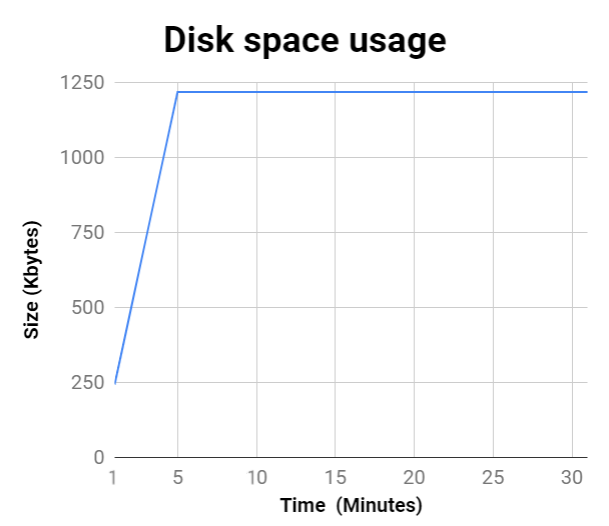
\includegraphics[scale=0.42]{evolucao_coleta_ieee.png}
\centering
\label{fig:evolucao_coleta}
\end{figure*}


A potential limitation of the solution proposed is that the pause of a container to collect data may, in principle, cause performance losses of the application being executed. 
%
To assess this impact, the times for copying the container memory were measured along the experiment.
%
The results are shown in the graph of Fig. \ref{fig:memoria_copia}.
%
Note that, after the application is initialized, the time for making a copy is very small, varying between 20 and 40 milliseconds. 
%
Especially for containers executing the engine of dynamic web pages, as is the case of the experiment in question, this latency can be not very perceptible by end users.

\begin{figure*}[htb!]
\footnotesize
\caption{Time for copying the container}
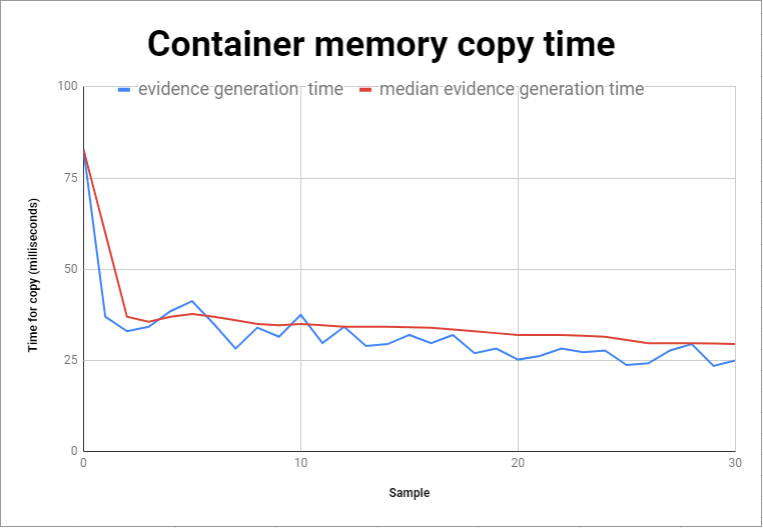
\includegraphics[scale=0.40]{memoria_copia_ieee.png}
\centering
\label{fig:memoria_copia}
\end{figure*}


Another concern is the time for transporting the evidence to the storage outside the cloud.
%
The evidence transport to the storage outside the cloud can take longer than generation interval, leading to evidence loss during transport. 
%
To assess this impact, the evidence transport times for storage outside the cloud were measured along the experiment, as shown by the results in the graph of Fig. \ref{fig:evidencia_transporte}.
%
The transport time is verified to stabilize after the window size is reached. 
%
The time for transporting evidence is approximately 30 seconds on average. 
%
The topology is a factor that may contribute both positively and negatively to the transport time. 
%
In this experiment, the evidence generator is in North America, whereas the physical machine where the evidence was transported to is in South America.

\begin{figure*}[htb!]
\footnotesize
\caption{Evidence transport time}
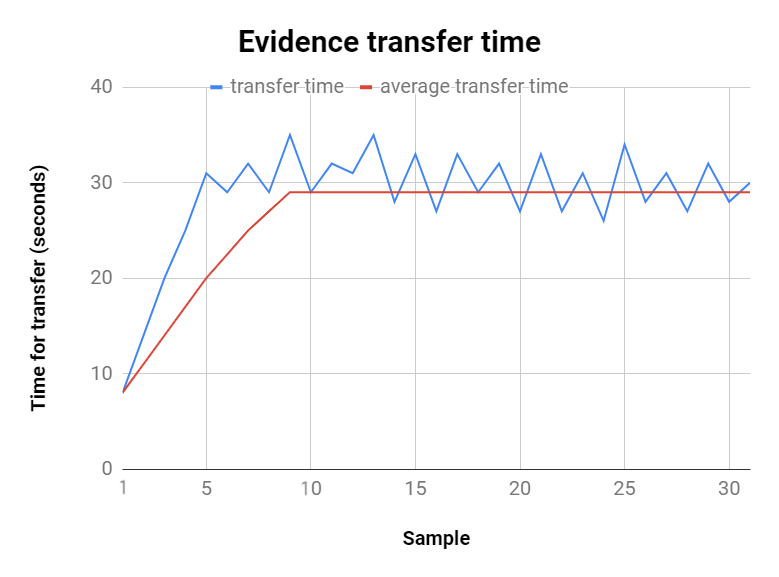
\includegraphics[scale=0.40]{evidencia_download_ieee.png}
\centering
\label{fig:evidencia_transporte}
\end{figure*}


\subsection{Limitations}

Since the solution described focuses on collecting memory information from the user space, it cannot access the kernel space. 
%
In principle, therefore, \fancyname does not provide support to malware investigation techniques based on information from the kernel space, such as comparing the information from the \textit{Process Environment Block} (PEB), which are in the user space, with information from the \textit{Virtual Address Descriptor}, which lies in the kernel space. 
%
Analyses of threats that directly manipulate the objects of the kernel (D.K.O.M – \textit{Direct Kernel Object Manipulation}) do not benefit from the solution proposed, either. 


% An example of a floating figure using the graphicx package.
% Note that \label must occur AFTER (or within) \caption.
% For figures, \caption should occur after the \includegraphics.
% Note that IEEEtran v1.7 and later has special internal code that
% is designed to preserve the operation of \label within \caption
% even when the captionsoff option is in effect. However, because
% of issues like this, it may be the safest practice to put all your
% \label just after \caption rather than within \caption{}.
%
% Reminder: the "draftcls" or "draftclsnofoot", not "draft", class
% option should be used if it is desired that the figures are to be
% displayed while in draft mode.
%
%\begin{figure}[!t]
%\centering
%\includegraphics[width=2.5in]{myfigure}
% where an .eps filename suffix will be assumed under latex, 
% and a .pdf suffix will be assumed for pdflatex; or what has been declared
% via \DeclareGraphicsExtensions.
%\caption{Simulation Results.}
%\label{fig_sim}
%\end{figure}

% Note that IEEE typically puts floats only at the top, even when this
% results in a large percentage of a column being occupied by floats.


% An example of a double column floating figure using two subfigures.
% (The subfig.sty package must be loaded for this to work.)
% The subfigure \label commands are set within each subfloat command,
% and the \label for the overall figure must come after \caption.
% \hfil is used as a separator to get equal spacing.
% Watch out that the combined width of all the subfigures on a 
% line do not exceed the text width or a line break will occur.
%
%\begin{figure*}[!t]
%\centering
%\subfloat[Case I]{\includegraphics[width=2.5in]{box}%
%\label{fig_first_case}}
%\hfil
%\subfloat[Case II]{\includegraphics[width=2.5in]{box}%
%\label{fig_second_case}}
%\caption{Simulation results.}
%\label{fig_sim}
%\end{figure*}
%
% Note that often IEEE papers with subfigures do not employ subfigure
% captions (using the optional argument to \subfloat[]), but instead will
% reference/describe all of them (a), (b), etc., within the main caption.


% An example of a floating table. Note that, for IEEE style tables, the 
% \caption command should come BEFORE the table. Table text will default to
% \footnotesize as IEEE normally uses this smaller font for tables.
% The \label must come after \caption as always.
%
%\begin{table}[!t]
%% increase table row spacing, adjust to taste
%\renewcommand{\arraystretch}{1.3}
% if using array.sty, it might be a good idea to tweak the value of
% \extrarowheight as needed to properly center the text within the cells
%\caption{An Example of a Table}
%\label{table_example}
%\centering
%% Some packages, such as MDW tools, offer better commands for making tables
%% than the plain LaTeX2e tabular which is used here.
%\begin{tabular}{|c||c|}
%\hline
%One & Two\\
%\hline
%Three & Four\\
%\hline
%\end{tabular}
%\end{table}


% Note that IEEE does not put floats in the very first column - or typically
% anywhere on the first page for that matter. Also, in-text middle ("here")
% positioning is not used. Most IEEE journals/conferences use top floats
% exclusively. Note that, LaTeX2e, unlike IEEE journals/conferences, places
% footnotes above bottom floats. This can be corrected via the \fnbelowfloat
% command of the stfloats package.

\section{Final Considerations}
\label{sec:conclusion}

Digital threats acting directly on the system memory do not usually leave traces in disk after their corresponding resources are removed, hindering later forensic analyses.
%
This problem is especially notable in cloud computing systems, in which the allocation and removal of virtualized resources (e.g. VMs and containers) are frequent.
%
This characteristic, together with aspects such as multitenancy and multi-jurisdiction of computational clouds, hinders evidence collection for investigating incidents.


In this scenario, the proposal presented aims to relate the memory photograph to its origin, using the calculated hash of the container image as a stored evidence identifier.
%
To prevent an excessive use of disk space, the volume of data stored uses a storage window, which allows describing the memory before and after an attack (e.g. memory injection).
%
Combined with a tool for identifying threats, these \fancyname characteristics make it a robust solution to provide evidence and thus make forensic analyses in the cloud viable.
%

As future work, we intend to analyze the containers memory of the same system using the collections made by \fancyname. 
%
With these results, the intention is to implement a more flexible tool, which dispenses with accessing the machine full memory, a common requirement of the current malware analysis tools. %(e.g., FROST \cite{Dykstra_FROST:2013} e Volatility Framework \cite{VolatilityFoundation2014}).



%\marcosR{As próximas frases, como escritas, são ``tiros no pé'': você fica falando das limitações que não são da sua proposta, mas sim do universo onde sua proposta se encaixa... Deixe a propaganda negativa para seus concorrentes fazerem, não para você... Refraseei para manter o mesmo conteúdo, mas de forma positiva em vez de negativa.}
%Apesar do sucesso em salvar a memória relacionadas ao contêiner e sua associação com a origem, não foi possível até o momento realizar uma análise das ameaças. 
%
%As ferramentas de análise de memória disponíveis no mercado necessitam que todo o conteúdo da memória da máquina esteja disponível para realização da análise. 
%
%Como é coletada apenas a memória relacionada aos processos, o ferramental não funciona. 
%
%É necessário o desenvolvimento de uma ferramenta que trabalhe sem a memória completa da máquina.

% trigger a \newpage just before the given reference
% number - used to balance the columns on the last page
% adjust value as needed - may need to be readjusted if
% the document is modified later
%\IEEEtriggeratref{8}
% The "triggered" command can be changed if desired:
%\IEEEtriggercmd{\enlargethispage{-5in}}

% references section

% can use a bibliography generated by BibTeX as a .bbl file
% BibTeX documentation can be easily obtained at:
% http://www.ctan.org/tex-archive/biblio/bibtex/contrib/doc/
% The IEEEtran BibTeX style support page is at:
% http://www.michaelshell.org/tex/ieeetran/bibtex/
\bibliographystyle{IEEEtran}
% argument is your BibTeX string definitions and bibliography database(s)
\bibliography{artigo-ieee}

% <OR> manually copy in the resultant .bbl file
% set second argument of \begin to the number of references
% (used to reserve space for the reference number labels box)

\end{document}


